\documentclass[letter, 10pt]{article}
\usepackage[utf8]{inputenc}
\usepackage[spanish]{babel}
\usepackage{amsfonts}
\usepackage{amsmath}
\usepackage[pdftex]{graphicx}
\usepackage{url}
\usepackage{hyperref}
%\usepackage[top=1.5cm,bottom=1.5cm,left=2cm,right=2cm,footskip=1.5cm,headheight=1.5cm,headsep=.5cm,textheight=3cm]{geometry}
\usepackage[top=1.5cm,bottom=1.5cm,left=2cm,right=2cm]{geometry}
\usepackage{fancyhdr}

\begin{document}
\title{\small{Universidad Técnica Federico Santa María\\Departamento de Informática}\\ \vspace{0.5cm}\huge{Diseño de Interfaces Usuarias}\\\Large{\emph{``Tarea 5 y 6''}}\\\Large{\emph{Perfil Cliente de Agendy.com}}}

\author{
\begin{tabular}{cc}
	\begin{tabular}{c}
		Cristián Maureira Fredes\\
		\url{cmaureir@inf.utfsm.cl}\\
		(Alumno)
	\end{tabular}
	&
	\begin{tabular}{c}
		Lioubov Dombrovskaia\\
		\url{lioubov.dombrovskaia@usm.cl}\\
		(Profesora)
	\end{tabular}
\end{tabular}}
\date{\today}
\maketitle


%Se debe usar:
%  Definición de perfil, tareas y frecuencias de Agendy.com
%  Experiencia como cliente de Agendy.com
%  Experiencia como profesional de Agendy.com
%     www.agendy.com/lioubov liuba@inf.utfsm.cl prueba2010
%  Patrones y métodos vistos en clases


%Nombre: Maureira-Tarea5y6.pdf
%Envío:  www.aula.usm.cl "Tarea 5 y 6: entrega en línea"
%Evaluación: Navegacion y Organizacion.

\section{Tarea}

\subsection{Introducción}
Para el desarrollo de la presente actividad se utilizó la siguiente información.~\footnote{Las imagenes utilizadas en el trabajo pueden no verse en una buena calidad, éstas pueden ser visualizadas mediante la página web \url{http://csrg.inf.utfsm.cl/~cmaureir/interfaces}}
\begin{itemize}
	\item Definición de perfil, tareas y frecuencias de Agendy.com
	\item Experiencia como cliente de Agendy.com
	\item Experiencia como profesional de Agendy.com
	\item Patrones y métodos
\end{itemize}
Para mayor información de la información con la que se comenzó a realizar el trabajo ver Anexo I~\ref{sec:anexo1}.

Es destacable el hecho de que el \emph{Cliente} del sistema poseía un conjunto de tareas que realizaba de forma
\emph{Ocasional} por lo cual la tarea de separar las actividades entre primarias y secundarias se realizó netamente
por la experiencia con el sistema y teniendo claro cuales eran las actividades con un grado de importancia superior
al resto.

\subsection{Árbol completo de navegación}
\begin{description}
	\item[Opciones Primarias:] \textbf{(1)} Consideraremos opciones primarias a las opciones de navegación
		más importantes en la página web.
	\item[Opciones Secundarias:] \textbf{(2)} Consideraremos opciones secundarias a las opciones que no son
		tan importantes en la navegación de la página web.
	% No mezclar verbos con sustantivos
	\begin{itemize}
		\item Home \textbf{(1)} 
		\item Citas
		\begin{itemize}
			\item Ver citas agendadas. \textbf{(1)}
			\item Modificar cita. \textbf{(2)}
			\item Cancelar cita.  \textbf{(2)} 
		\end{itemize}
		\item Profesionales
		\begin{itemize}
			\item Búsqueda Profesionales
			\begin{itemize}
				\item Agendar cita.\textbf{(1)} 
				\item Consultar ubicación  \textbf{(2)}
				\item Mandar mensaje  \textbf{(2)}
			\end{itemize}
		\end{itemize}
		\item Mi Cuenta~\footnote{Asumiendo que el usuario está logueado en el sistema}
		\begin{itemize}
			\item Modificar Perfil  \textbf{(2)}
			\item Restablecer contraseña  \textbf{(2)}
		\end{itemize}
		\item Ayuda
		\begin{itemize}
			\item Mandar mensaje a soporte  \textbf{(2)}
		\end{itemize}
	\end{itemize}
\end{description}
%
% PAGINA PROFESIONAL
%
\subsection{Prototipo Página Principal Profesional}
\begin{itemize}
	\item Opciones de navegación primarias (e.g: www.agendy.com/lioubov), no es necesario autentificarse.
\end{itemize}

La presente página se despliega una vez que el usuario accede al menú \emph{Profesionales $>$ Búsqueda Profesionales}
y se ingresa el nombre del profesional.

Para ayudar a que el usuario sepa en el lugar que se encuentra actualmente,
se utiliza el patrón de \emph{migas de pan} y además la \emph{navegación global} ya que el menú de la página siempre es el mismo.

La página además presenta el \emph{Nombre},\emph{Profesión} y \emph{Descripción}, del profesional,
para que el usuario logre conocer la persona de la cual puede que solicite un servicio.

Hay dos botones \emph{grandes} que intentan resaltar dos opciones principales al estar en la página del profesional
determinado, \emph{Reservar} un servicio determinado y \emph{Contacto}, donde se le podrá enviar un mensaje personal
al profesional.


\begin{center}
	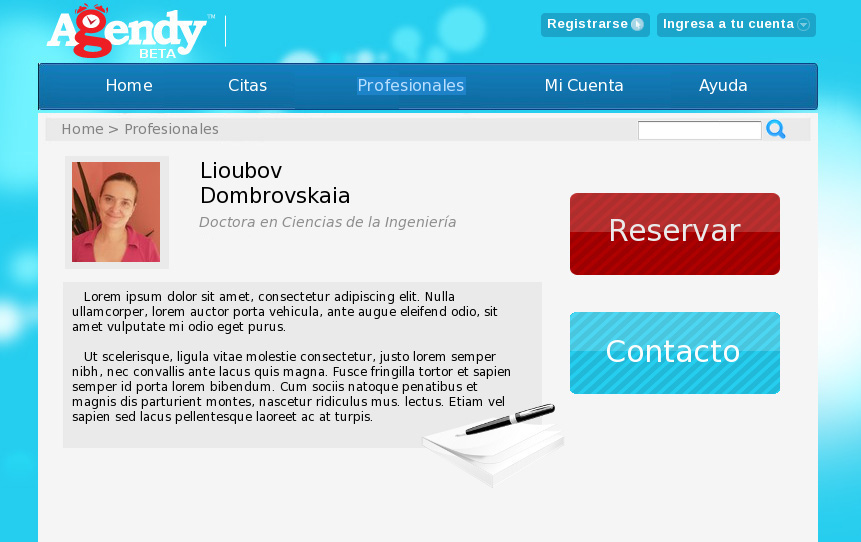
\includegraphics[width=18cm]{images/2}
\end{center}

%
% PROTOTIPO AGENDAR CITA
%
\subsection{Prototipo Página Tarea}
\begin{itemize}
	\item Agendar cita:
	\begin{itemize}
		\item Definir opciones de navegación
		\begin{itemize}
			\item Enlaces, Menús, Botones, etc.
		\end{itemize}
		\item Organizar espacio y secuencia de páginas
	\end{itemize}
\end{itemize}

\subsubsection{Paso 1 - Seleccionar Servicio}

En éste primer paso, el usuario podrá seleccionar el servicio que deseado haciendo \emph{click} en él.
Se pensaron varias alternativas para mostrar ésta información, \emph{combobox}, \emph{checkbox}, \emph{buttons},
pero se llegó a la conclusión de mostrar una tabla con todos los servicios y sus detalles como duración y precio.~\footnote{
Realice una encuesta a 10 personas, con 4 implementaciones distintas de ésta vista, con los elementos anteriormente mencionados,
resultando ganador la tabla, que a modo personal, también era la que más me acomodaba.}

Con respecto a los patrones, las \emph{migas de pan} siguen estando presentes, además se encuentran tres iconos circulares
que le informan al usuario en que parte de la tarea \emph{agendar cita} se encuentra.

Eventualmente si el profesional tiene muchos servicios el tamaño de la tabla será controlado por un \emph{scrollbar}

El usuario puede hacer click en \emph{Continuar} para seguir al siguiente paso.

\begin{center}
	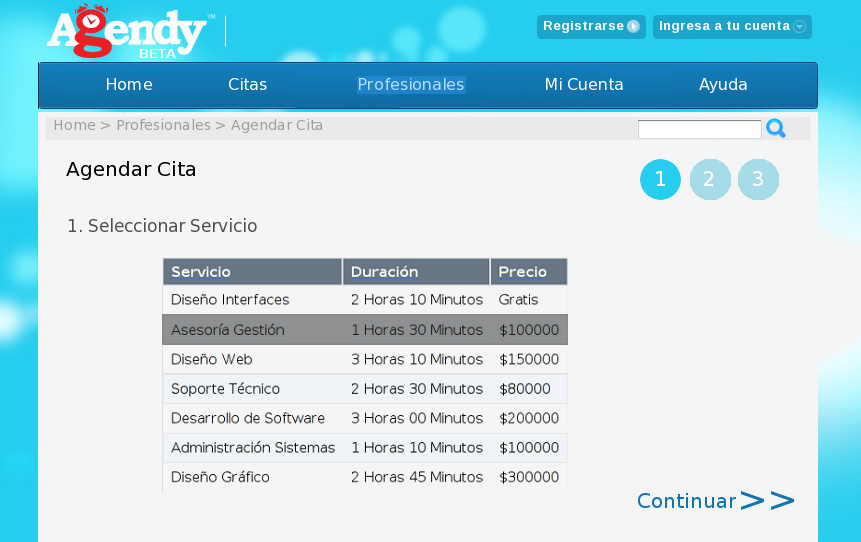
\includegraphics[width=18cm]{images/3_1}
\end{center}
\newpage
\subsubsection{Paso 2 - Seleccionar Fecha y Hora}
En el segundo paso, el usuario tiene dos elementos a seleccionar,
el primero de ellos es el calendario de la izquierda para seleccionar la fecha en la cual necesita el servicio,
por otro lado en la derecha se encuentra una lista con los horarios disponibles para dicho servicio.
Los horarios que ya estén seleccionados por otra persona no se desplegaran en la tabla.~\footnote{El criterio para el ``cómo'' desplegar los horarios,
fue basado en los mismos criterios para la selección se los servicios.}

El usuario también puede perfectamente volver al paso anterior por si desea hacer alguna modificación.

\begin{center}
	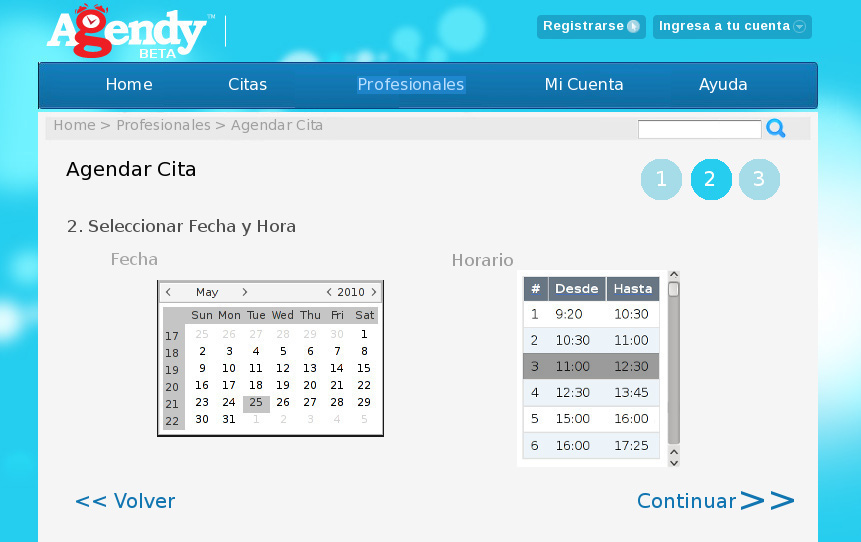
\includegraphics[width=18cm]{images/3_2}
\end{center}
\newpage
\subsubsection{Paso 3 - Confirmación}
En esta última vista, el usuario recibe un resumen de toda la información seleccionada en los pasos anteriores,
para que puede verificar si todo está correcto a sus necesidades.

Al igual que los pasos previos, el usuario puede finalizar la tarea o volver a un paso previo,
sin perder la información seleccionada.

\begin{center}
	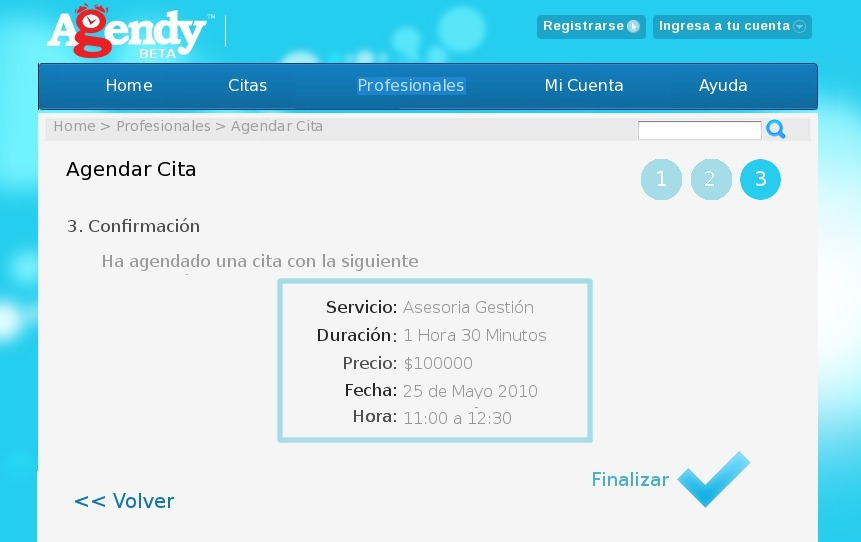
\includegraphics[width=18cm]{images/3_3}
\end{center}

\subsubsection{Conclusiones generales}
Los pasos para realizar la tarea previa tienen una estructura igual al momento de desplegar información al usuario.
Primero que todos podemos notar que existen espacios entre los distintos títulos, para realizar una jerarquía aparte de la notoria
que es con respecto al tamaño y color de las fuentes.

Existe un patrón utilizado que no está dentro de los vistos en clases, que es el de tener una navegación estilo \emph{wizard}, consiguiendo así
que el usuario vaya ingresando la información necesaria secuencialmente y de forma ordenada. Los patrones anteriormente explicados y utilizados son
las \emph{migas de pan} y la \emph{navegación global}.

Para el flujo visual del usuario, se utiliza  el patrón de \emph{balance diagonal}, pues si nos damos cuenta tenemos una jerarquía desde el logo de la empresa
hasta el botón continuar, pasando obviamente por los campos donde el usuario debe ingresar o seleccionar la información requerida.


%
% ANEXO I
%
\newpage
\section{Anexo I}
\label{sec:anexo1}
En el presente anexo se presenta la información que se tuvo de precedente para realizar el trabajo.

Primero que todo necesitamos tener claro los usuarios de la presente página web, por lo que hay
una descripción considerando las características necesarias de cada uno.

Luego tenemos una lista de las tareas y la frecuencia con la que se realizan, ya sea por parte de los clientes
como de los profesionales. En este caso se utilizaron sólo las tareas del cliente.

Finalmente se tiene una lista de los patrones recomendados para realizar una óptima navegación web,
de los cuales algunos fueron seleccionados para realizar el prototipo.


\subsection{Definición de usuarios y tareas de Agendy.com}
\begin{itemize}
	\item Profesional: aquella persona que necesita agendar sus servicios
	\begin{itemize}
		\item Experiencia computacional - media
		\item Conocimiento del dominio - alto
		\item Experiencia con el sistema - media
	\end{itemize}
	\item Cliente: aquella persona que requiere atenderse con el profesional
	\begin{itemize}
		\item Experiencia computacional - media
		\item Conocimiento del dominio - media
		\item Experiencia con el sistema - baja	
	\end{itemize}
\end{itemize}
\subsection{Frecuencias de las Tareas}
\begin{tabular}{|l|l|l|}
\hline
{\bf Tarea} & {\bf Profesional} & {\bf Cliente} \\\hline
Registrarse como profesional & 1 vez & - \\\hline
Registrarse como cliente & - & 1 vez \\\hline
Administrar horario de atención & Ocasional & - \\\hline
Ver citas agendadas (por periodo) & Frecuente & - \\\hline
Ver cita agendada & - & Ocasional \\\hline
Modificar perfil profesional & Ocasional & - \\\hline
Modificar perfil personal & - & Ocasional \\\hline
Agendar cita & Frecuente & Ocasional \\\hline
Modificar cita & Frecuente & Ocasional \\\hline
Cancelar cita & Frecuente & Ocasional \\\hline
Consultar ubicación del profesional & - & Ocasional \\\hline
Buscar profesional en el directorio & - & Ocasional \\\hline
Restablecer contraseña & - & Ocasional \\\hline
Mandar mensaje a soporte & Ocasional & Ocasional \\\hline
Mandar mensaje a profesional & - & Ocasional \\\hline
\end{tabular}
\begin{itemize}
	\item Frecuente: la tarea se realiza al menos 2 veces al día.
	\item Ocasional: la tarea se realiza a lo más 5 veces al mes.
\end{itemize}
\subsection{Patrones}
\begin{tabular}{p{0.4\textwidth} p{0.4\textwidth}}

\begin{itemize}
	\item Claros puntos de entrada
	\item Navegación Global
	\item Concentrador
	\item Pirámide
	\item Panel Modal
	\item Mapa de secuencia
\end{itemize}
&
\begin{itemize}
	\item Migas de pan
	\item Scroll con anotaciones
	\item Secciones en colores
	\item Transición animada
	\item Escotilla de escape
\end{itemize}
\\
\end{tabular}

\vfill \hfill CM/\LaTeX
\end{document} 
